
\section{Resultados}

Las estrategias de control implementadas fueron probadas con dos casos de prueba: bajo una referencia estática en un punto arbitrario y bajo el seguimiento de una trayectoria circular.

El caso bajo una referencia estática se evaluó el tiempo de estabilización y el error en estado estable y en el caso de seguimiento de trayectorias se evaluó qué tan robusto es el sistema y el comportamiento del mismo fuera del punto de linealización.

Los controles que fueron implementados 
\subsection{Control PD}

\subsubsection{Bajo patrón de movimiento}
\begin{figure}[h]
    \centering
    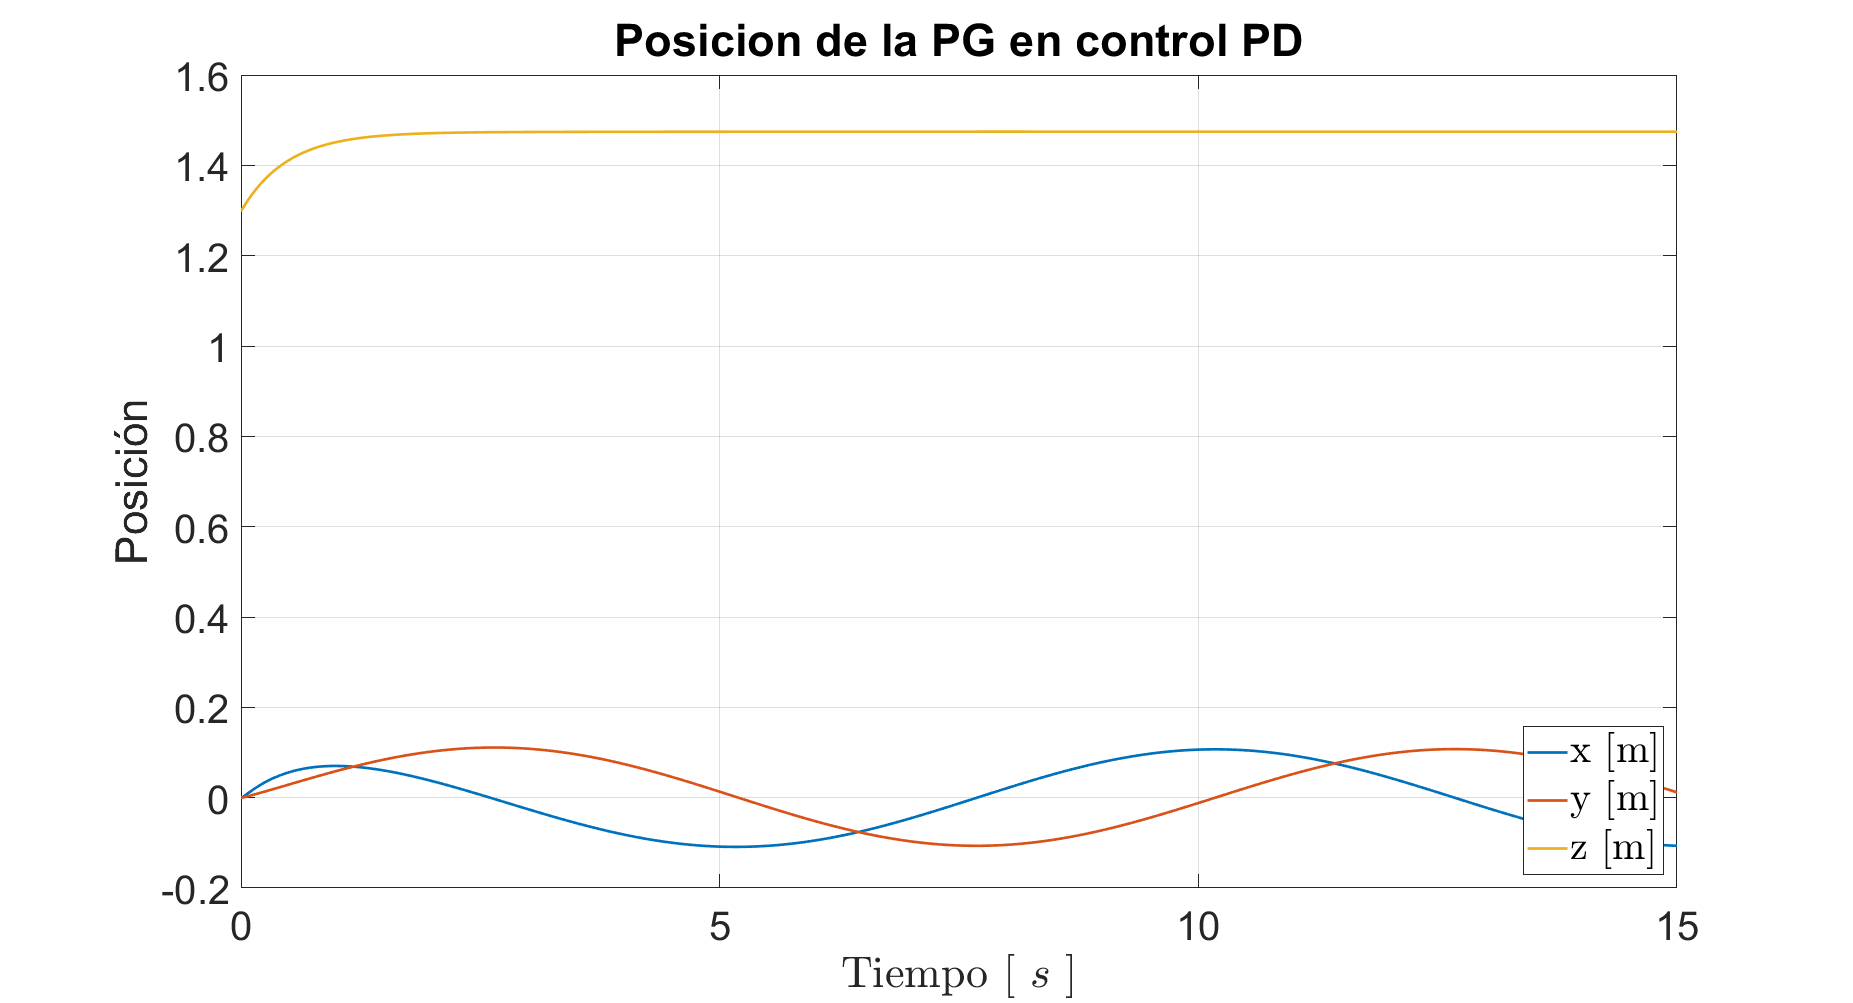
\includegraphics[width=0.4\textwidth]{posPD.png}
    \caption{Posición del sistema - PD.}
    \label{fig:PD position}
\end{figure}

\begin{figure}[h]
    \centering
    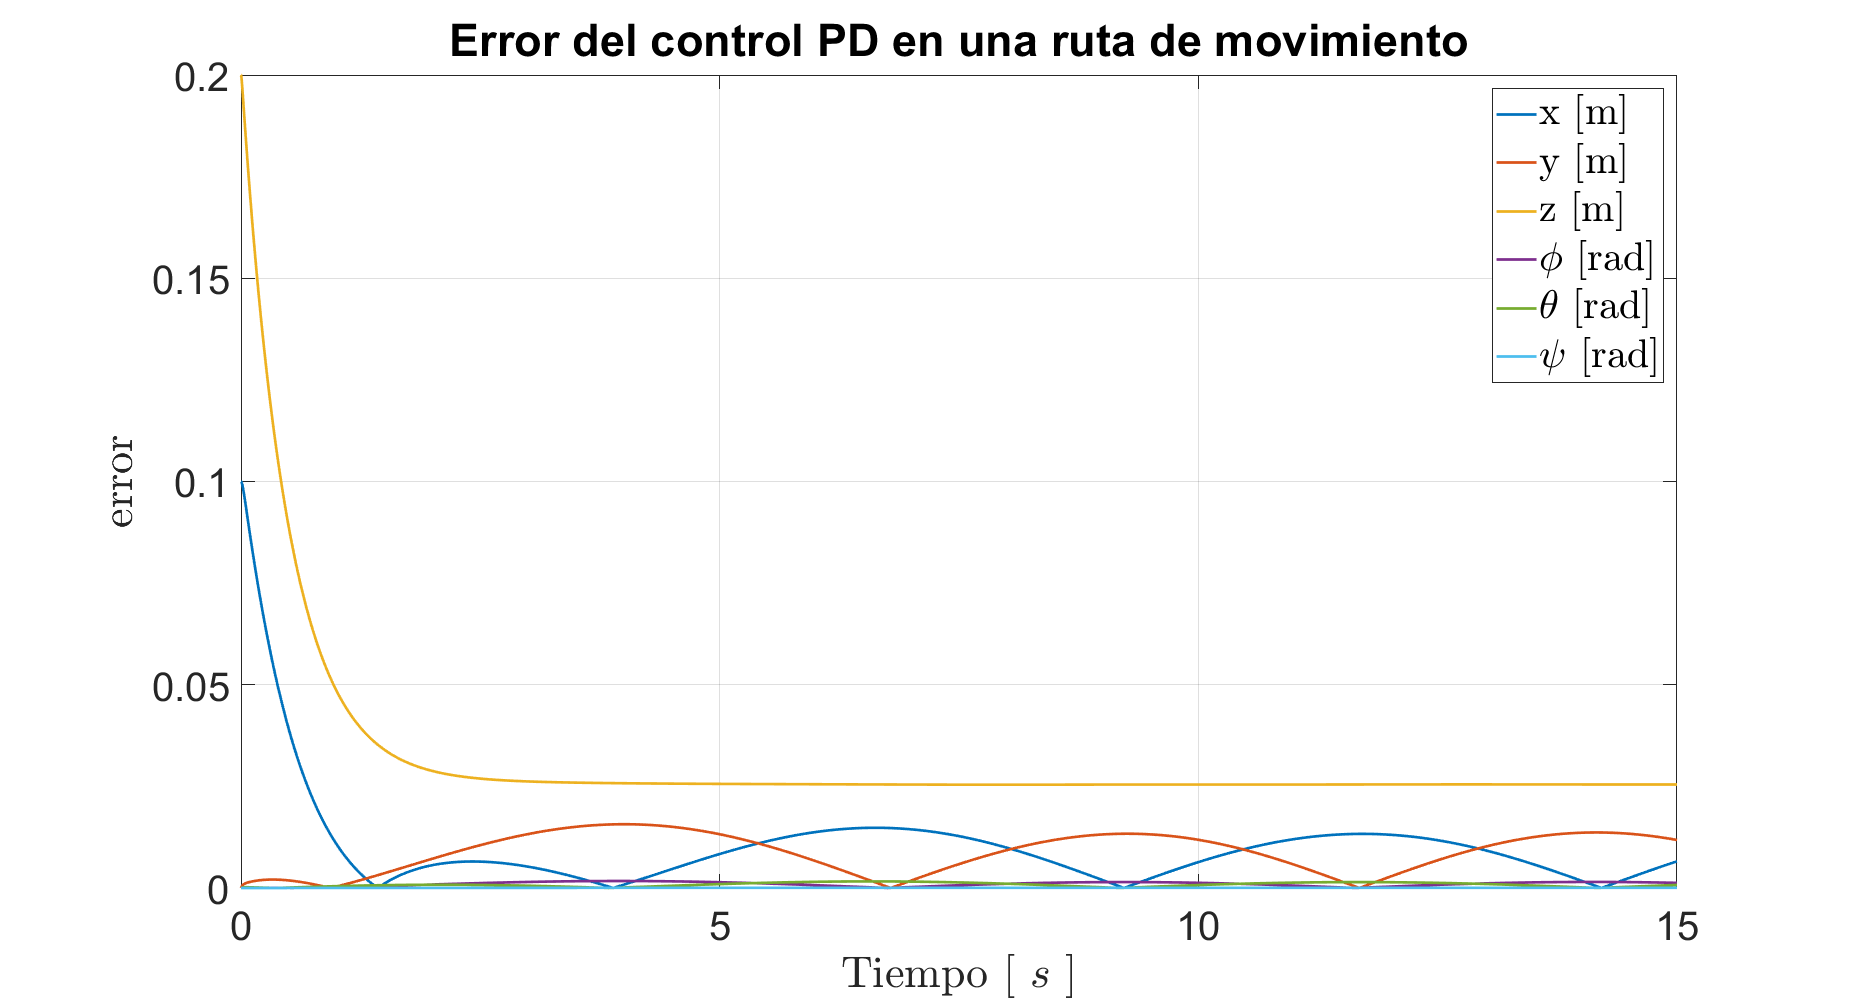
\includegraphics[width=0.4\textwidth]{errorPD.png}
    \caption{Error del sistema - PD.}
    \label{fig:PD error}
\end{figure}

\subsubsection{Bajo una referencia estática}

\begin{figure}[htb]
    \centering
    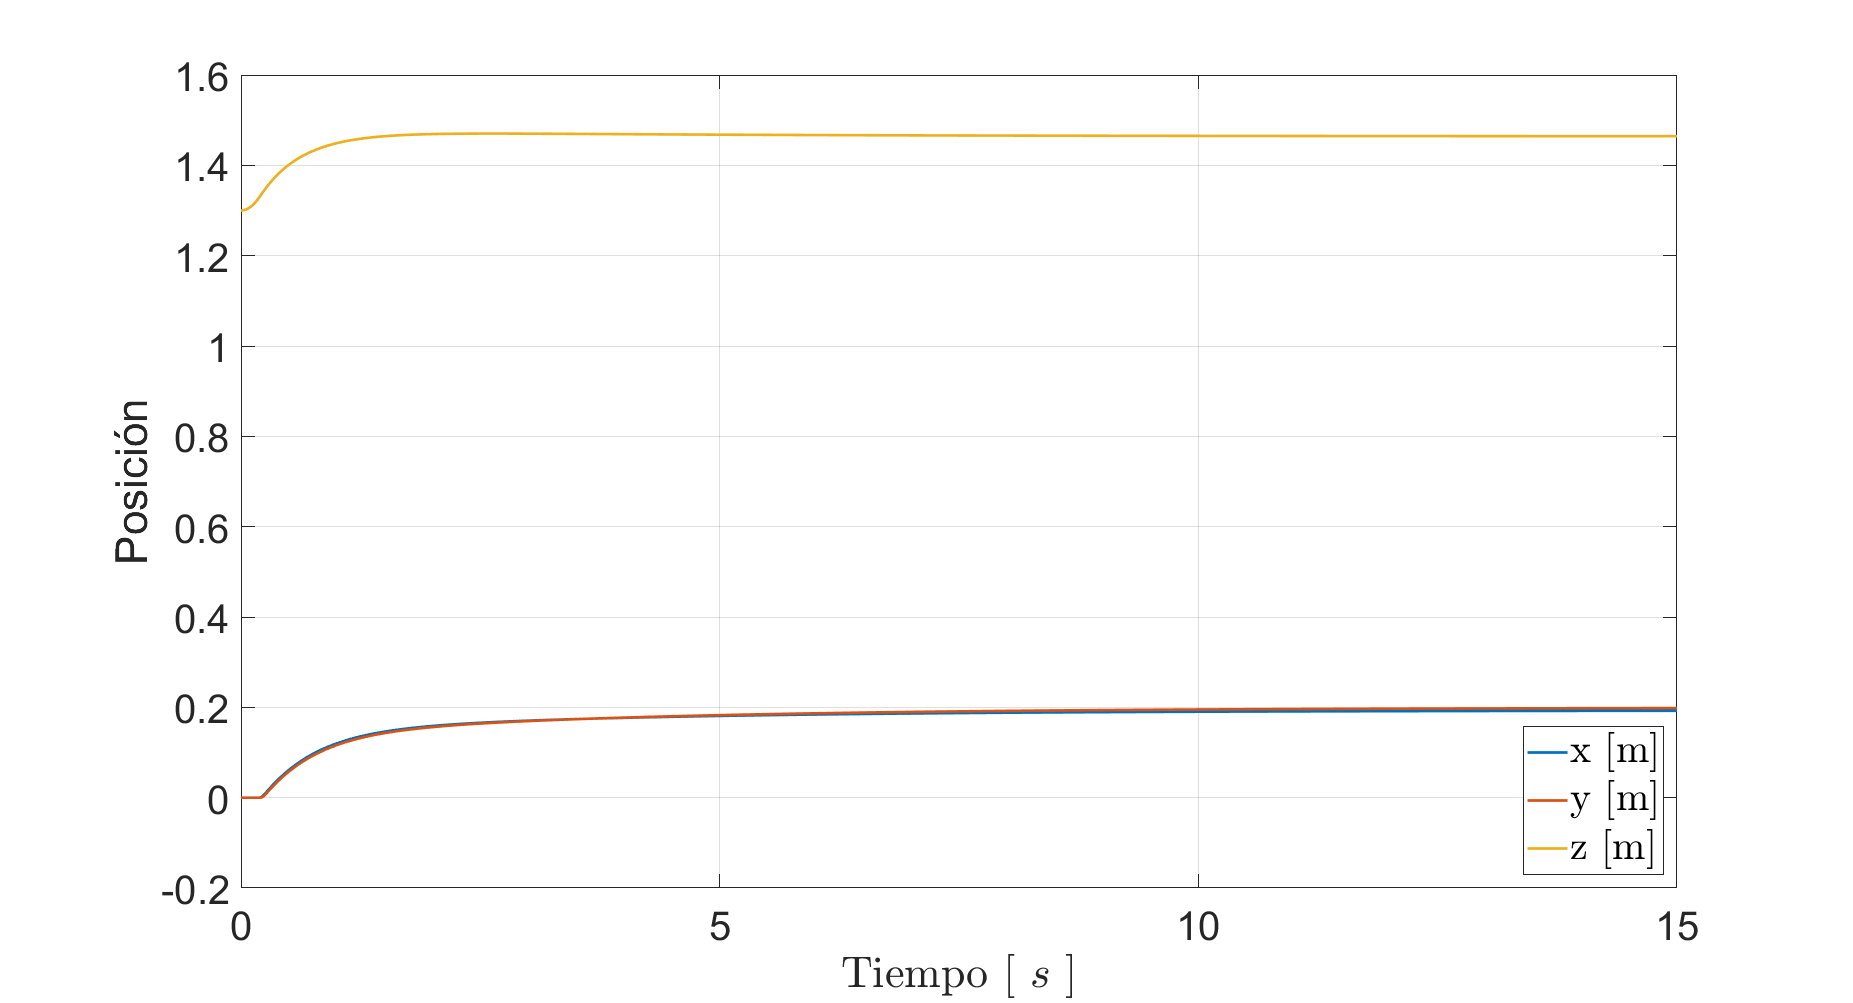
\includegraphics[width=0.4\textwidth]{posPDe.png}
    \caption{Posición del sistema - PD.}
    \label{fig:PD position}
\end{figure}

\begin{figure}[htb]
    \centering
    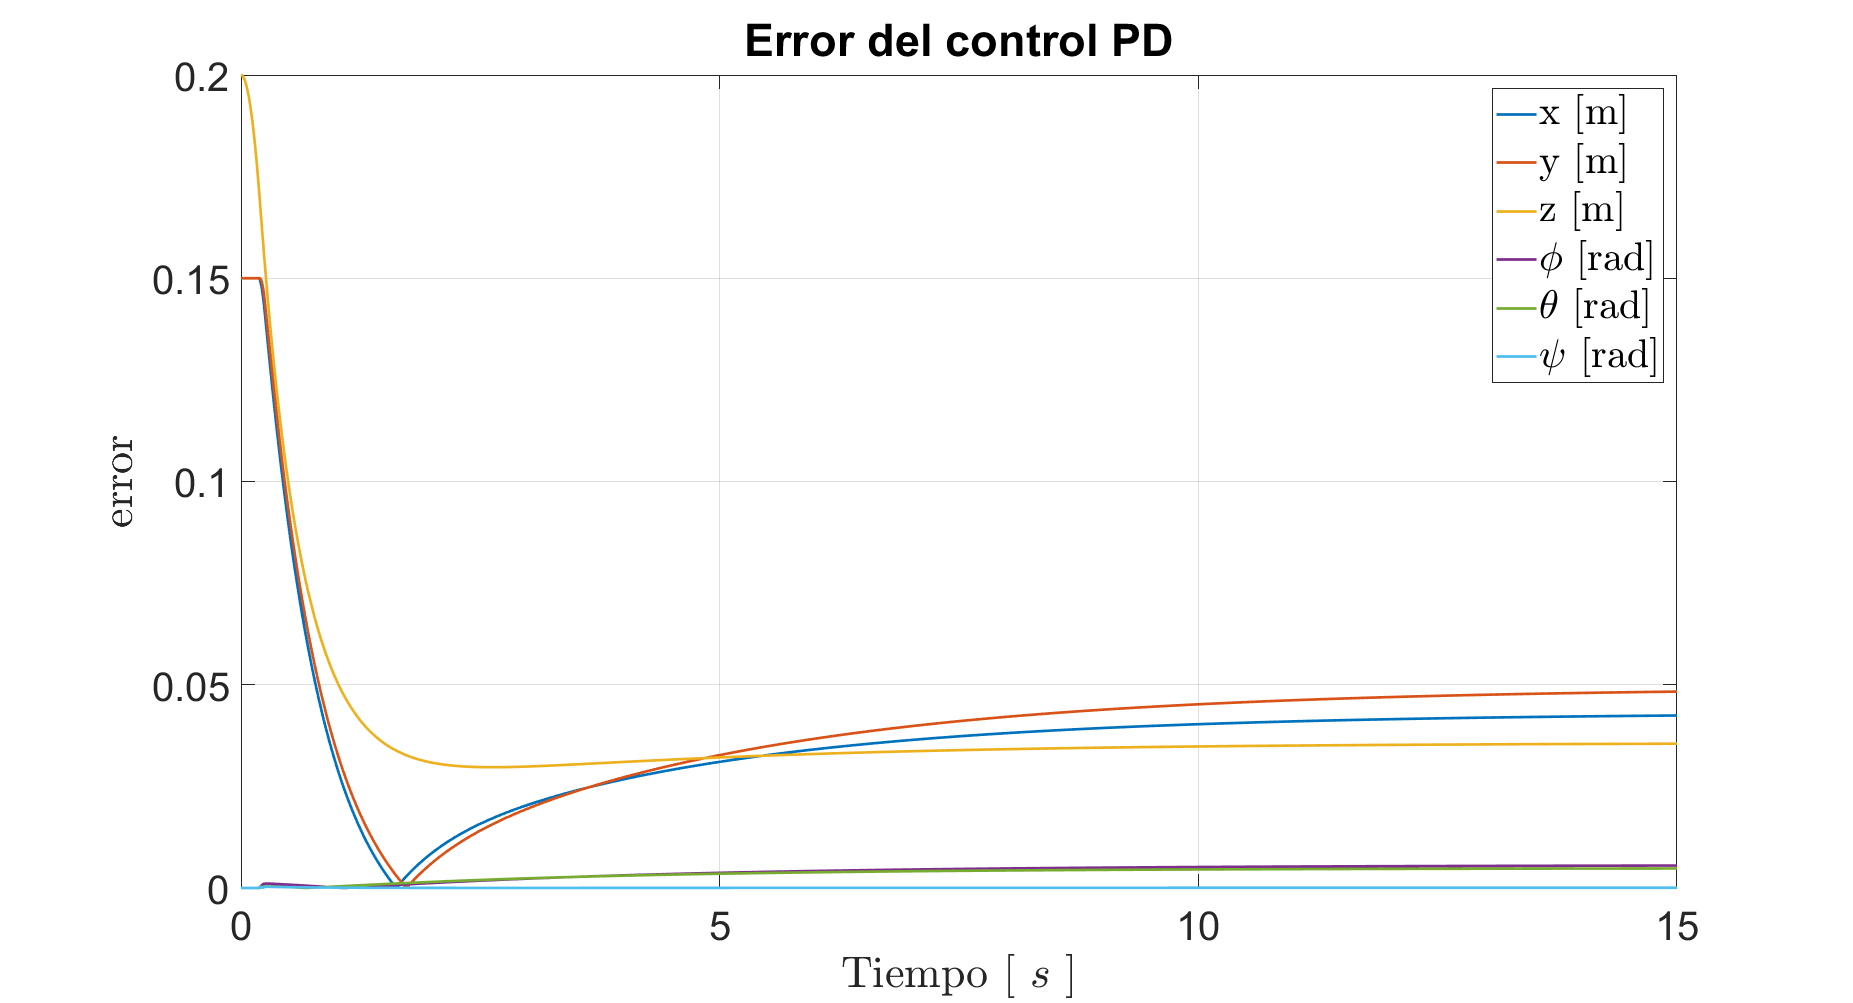
\includegraphics[width=0.4\textwidth]{errorPDe.png}
    \caption{Error del sistema - PD.}
    \label{fig:PD error}
\end{figure}


\subsection{Control PD+G}

\subsubsection{Bajo patrón de movimiento}

\begin{figure}[htb]
    \centering
    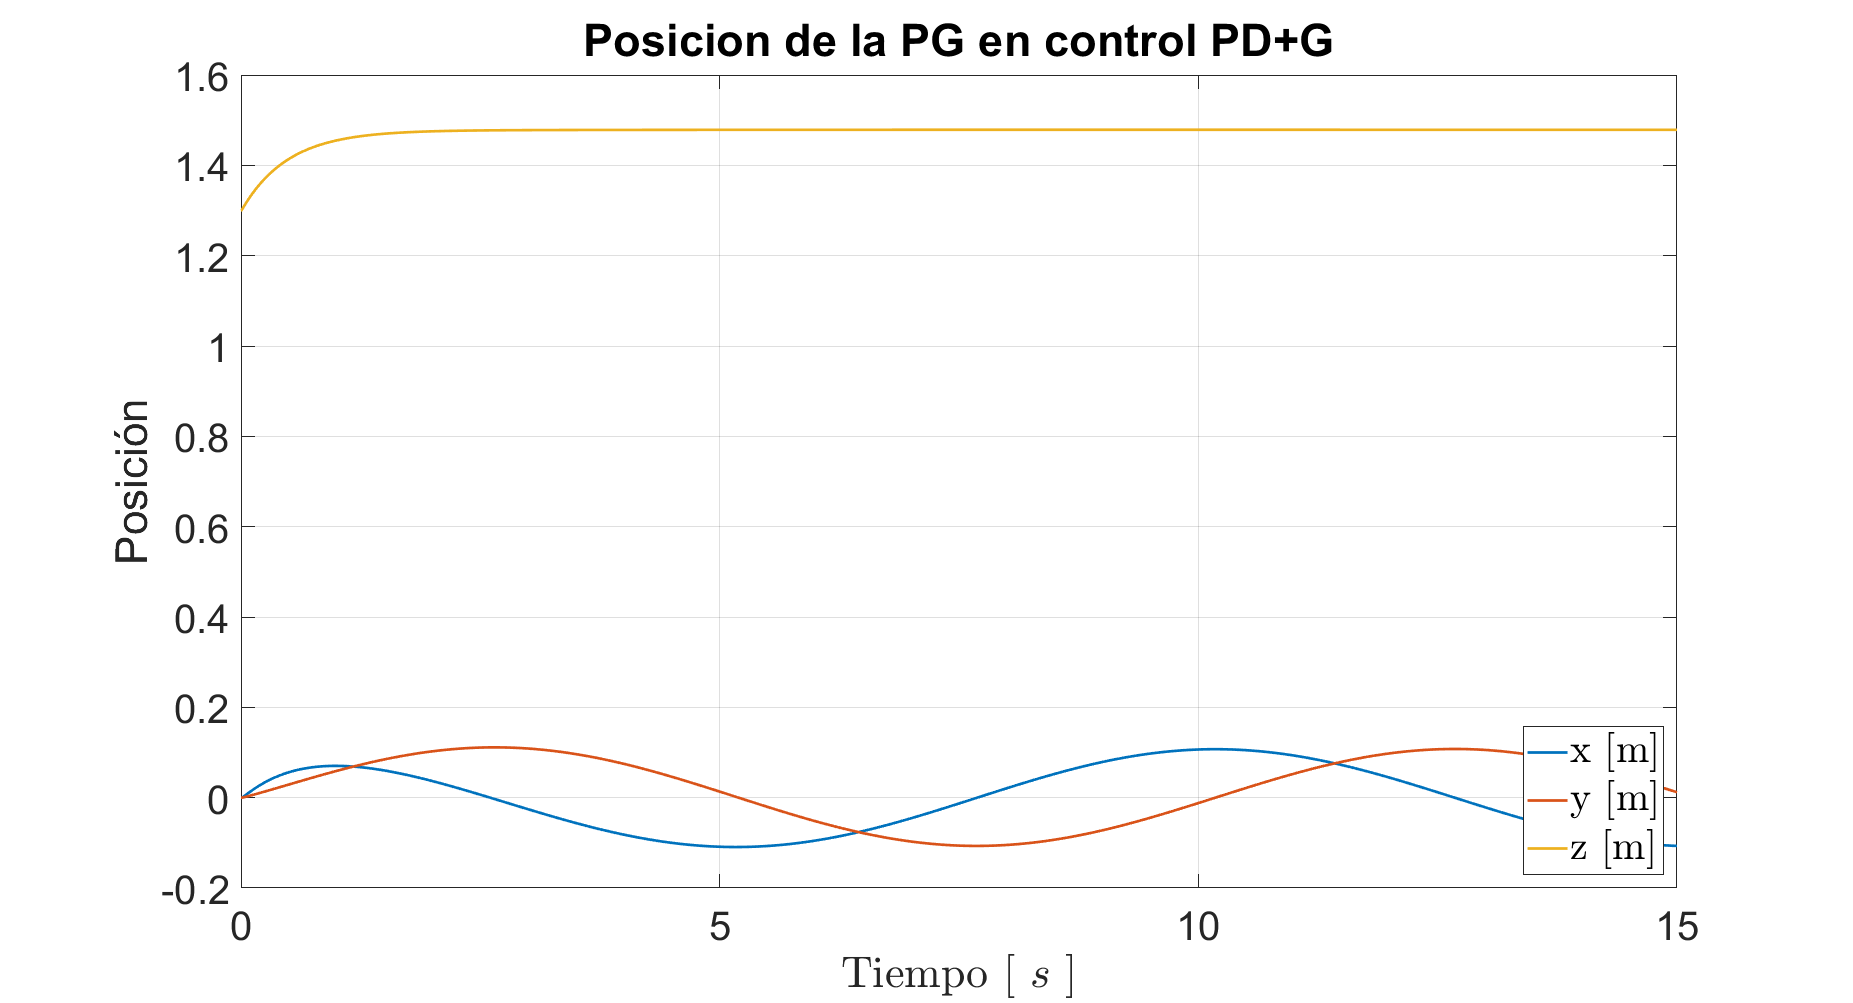
\includegraphics[width=0.4\textwidth]{posPDpG.png}
    \caption{Posición del sistema - PD+G.}
    \label{fig:PDG position}
\end{figure}

\begin{figure}[htb]
    \centering
    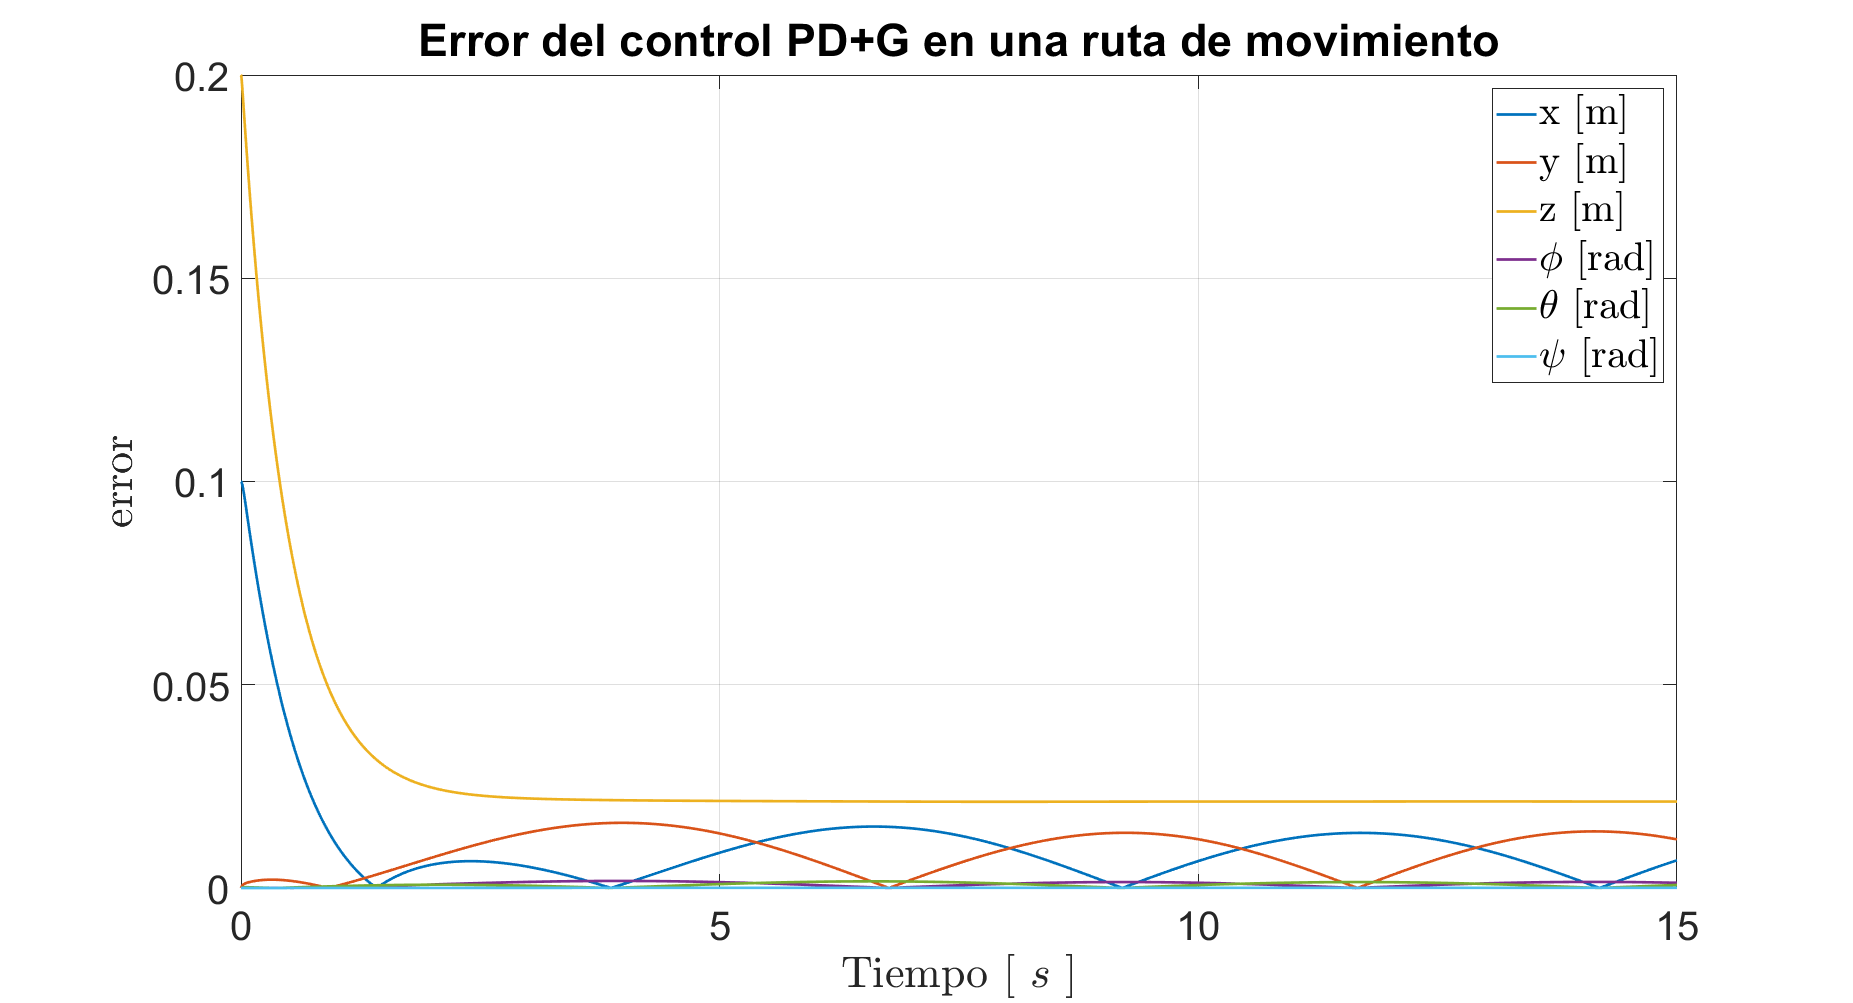
\includegraphics[width=0.4\textwidth]{errorPDpG.png}
    \caption{Error del sistema - PD+G.}
    \label{fig:PDG error}
\end{figure}

\subsubsection{Bajo una referencia estática}

\begin{figure}[htb]
    \centering
    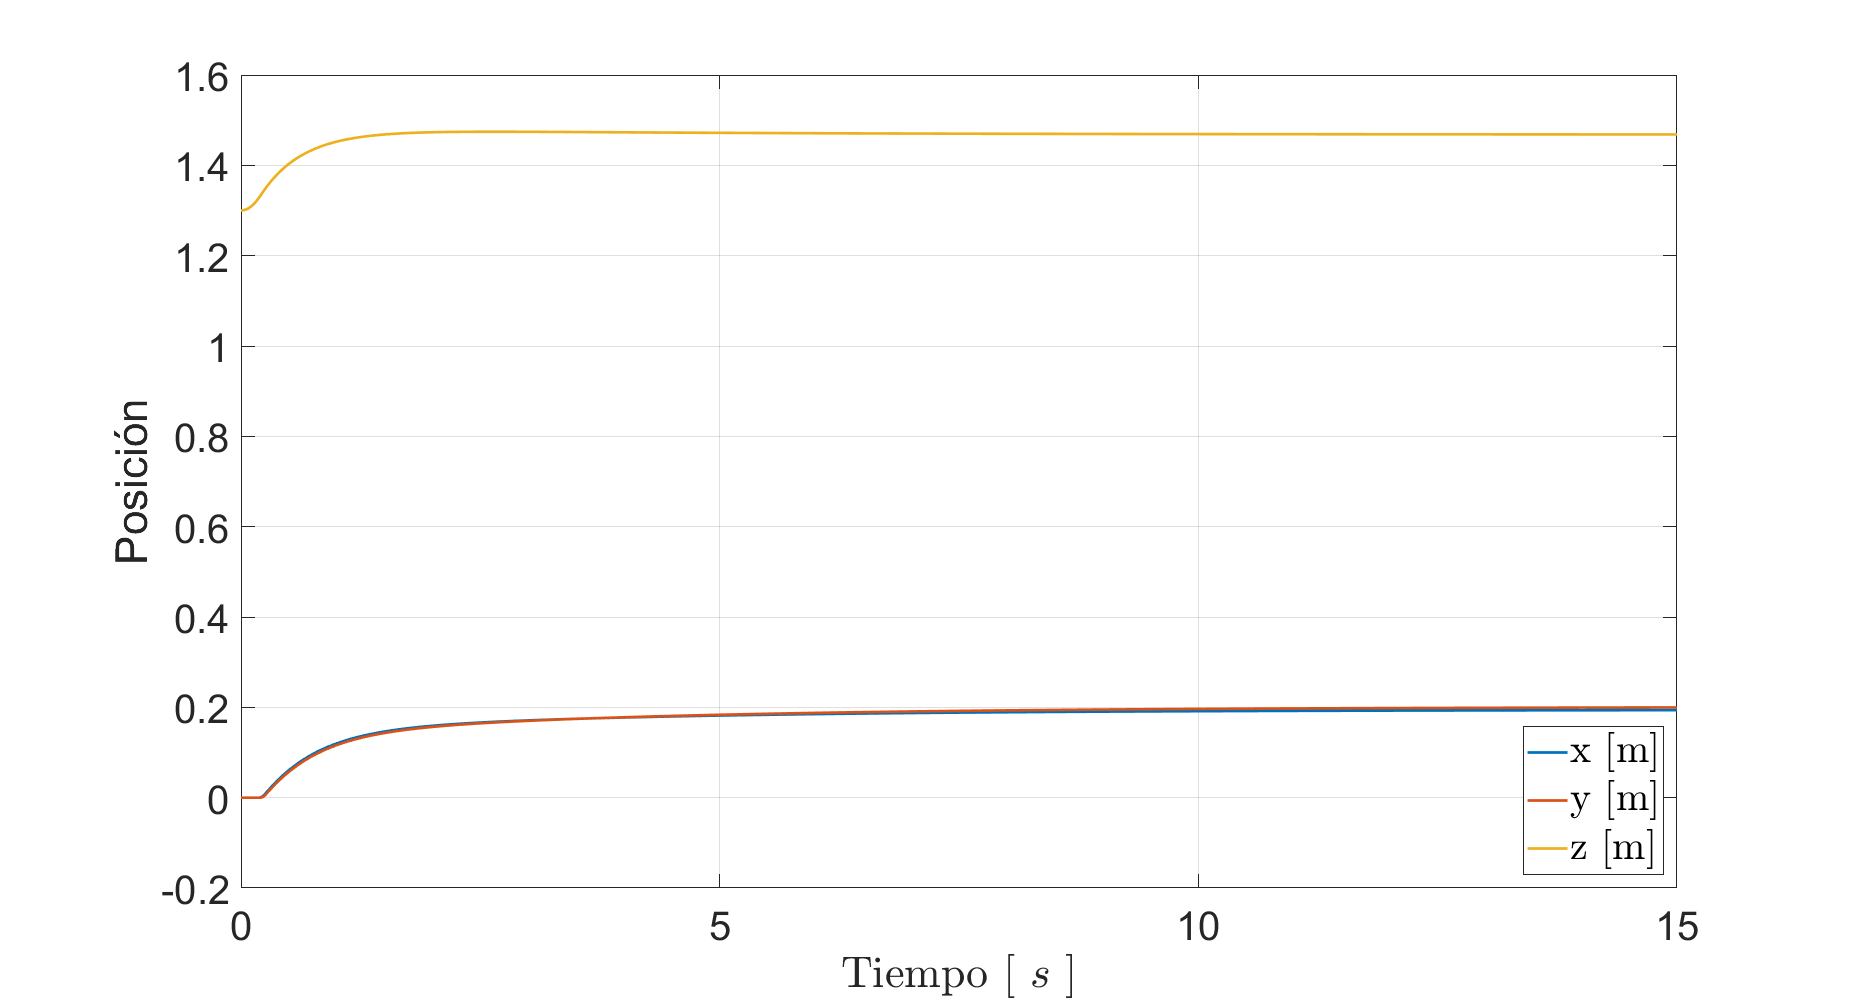
\includegraphics[width=0.4\textwidth]{posPDpGe.png}
    \caption{Posición del sistema - PD+G.}
    \label{fig:PDG position}
\end{figure}

\begin{figure}[htb]
    \centering
    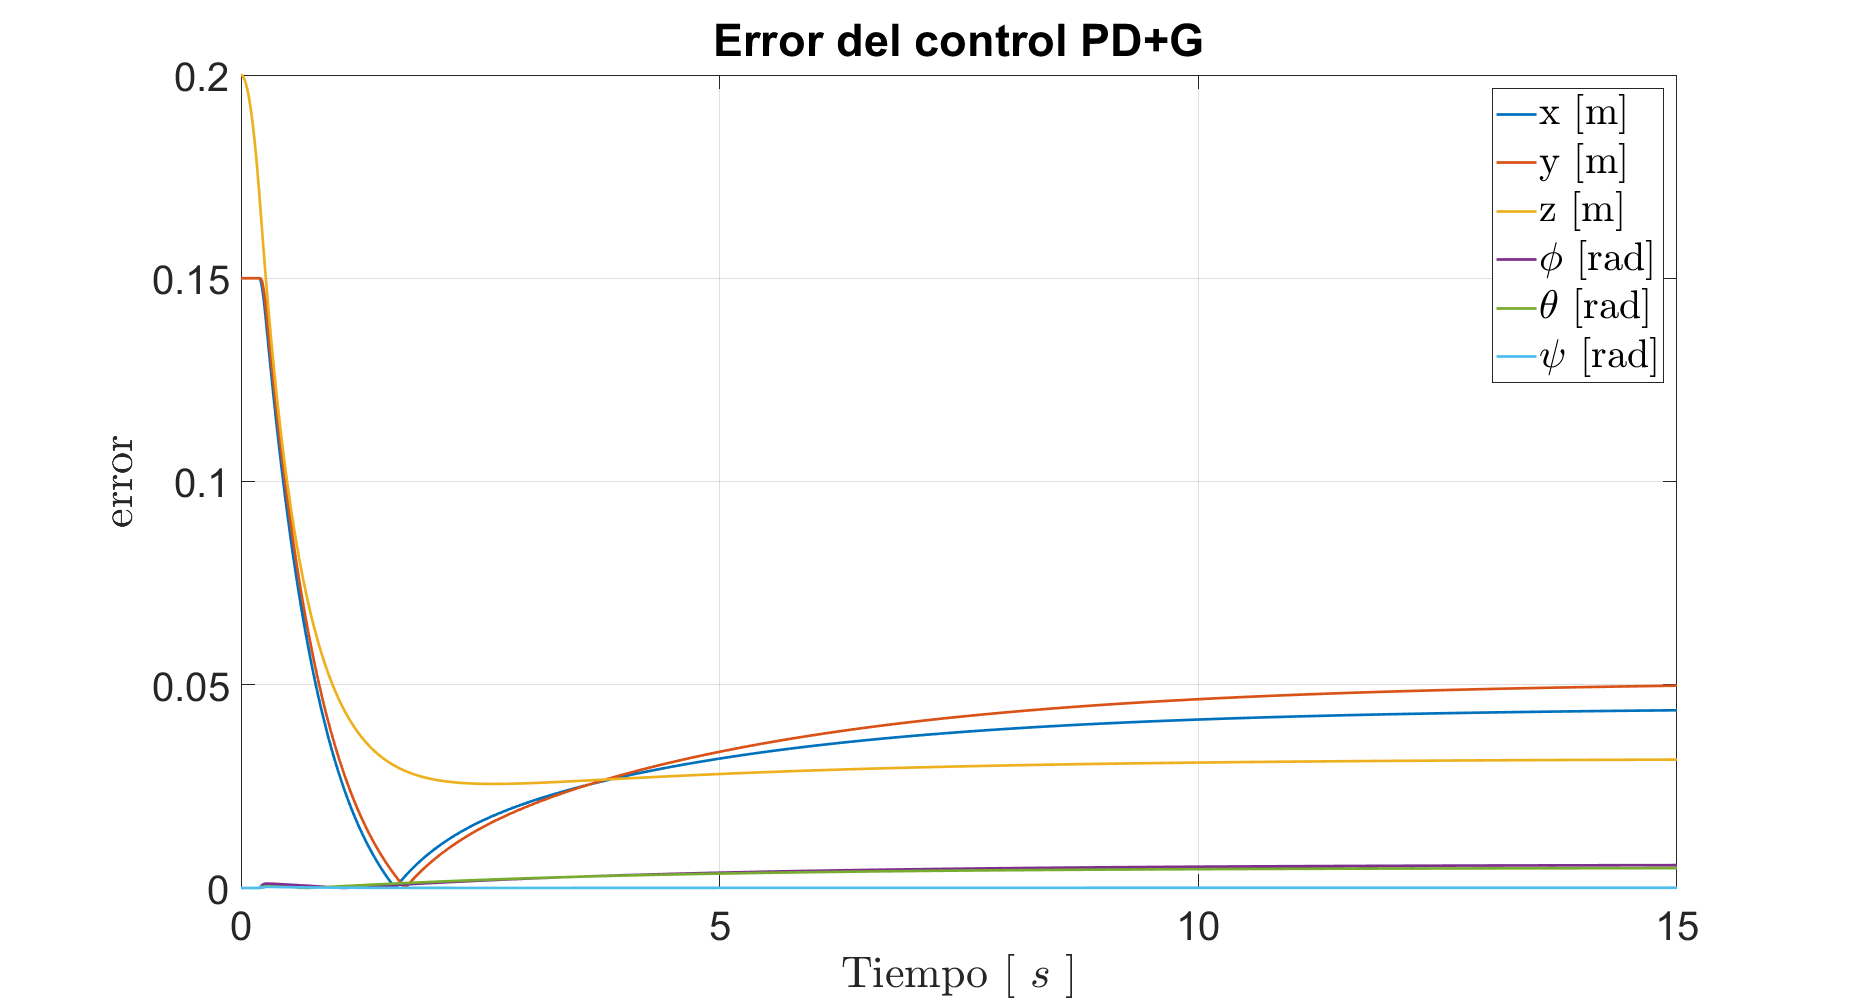
\includegraphics[width=0.4\textwidth]{errorPDpGe.png}
    \caption{Error del sistema - PD+G.}
    \label{fig:PDG error}
\end{figure}


\subsection{Control PID}

\subsubsection{Bajo patrón de movimiento}

\begin{figure}[htb]
    \centering
    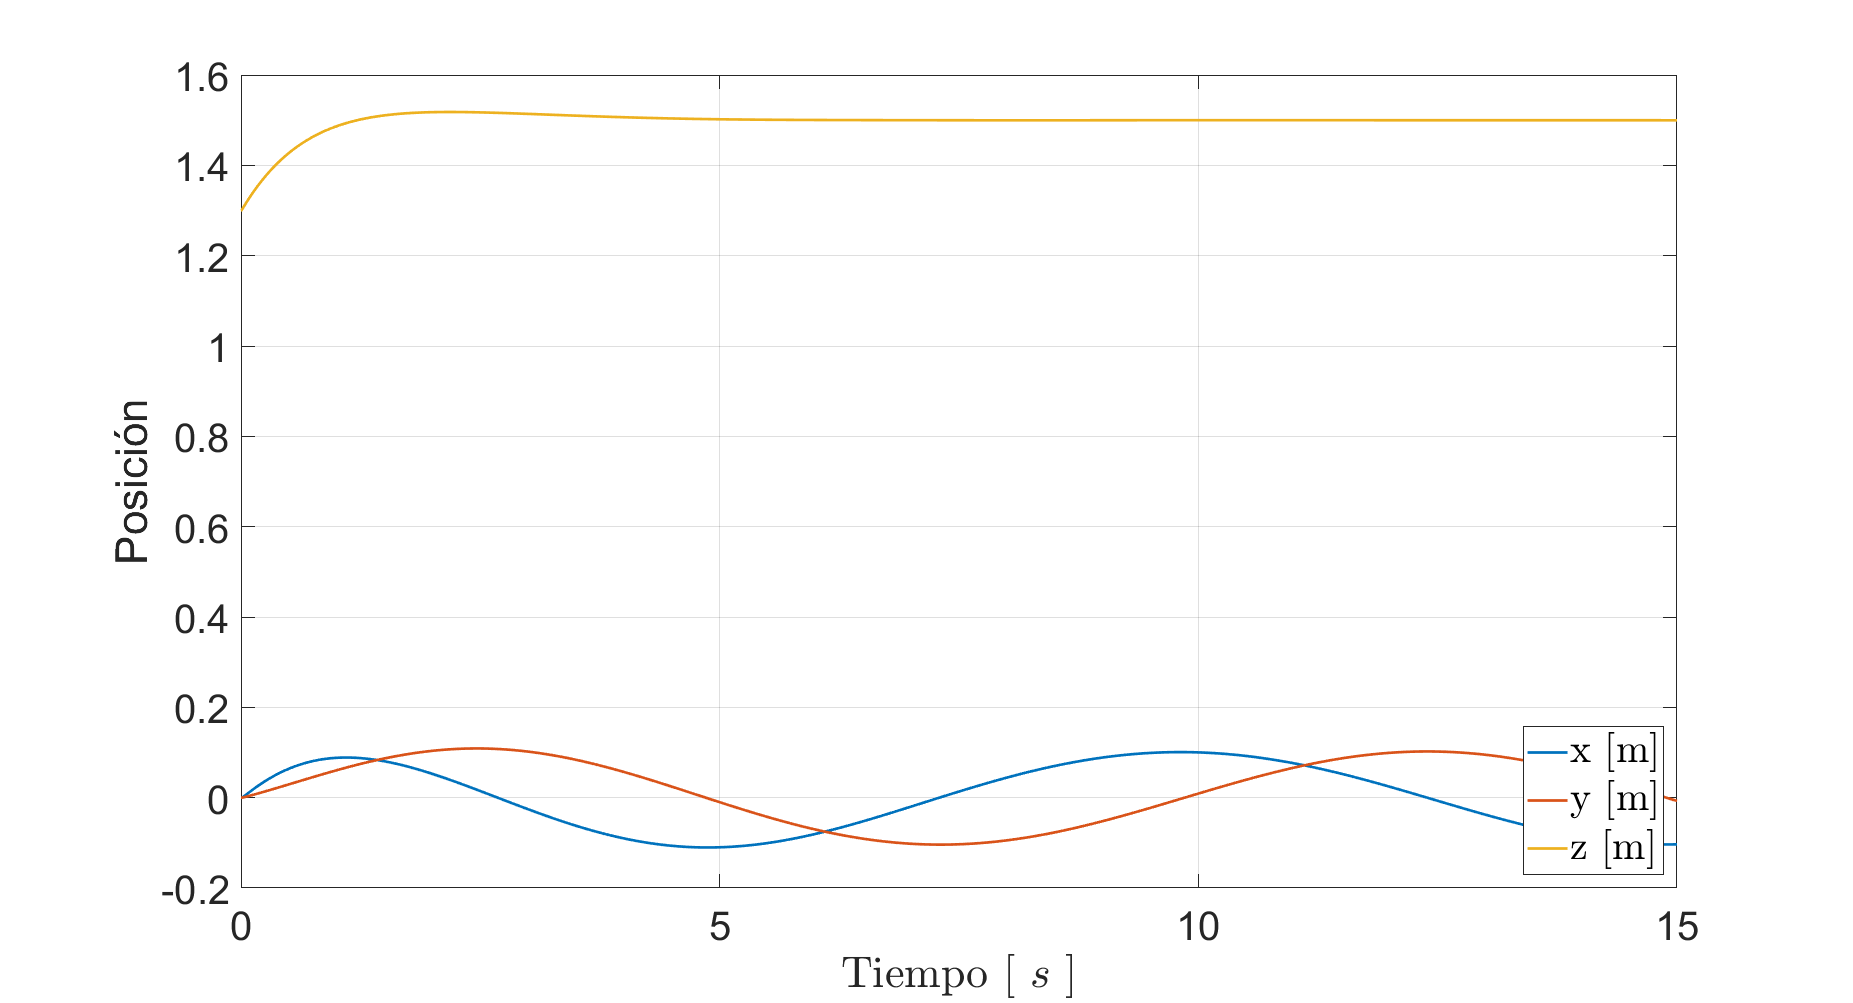
\includegraphics[width=0.4\textwidth]{posPID.png}
    \caption{Posición del sistema - PID.}
    \label{fig:PID position}
\end{figure}

\begin{figure}[htb]
    \centering
    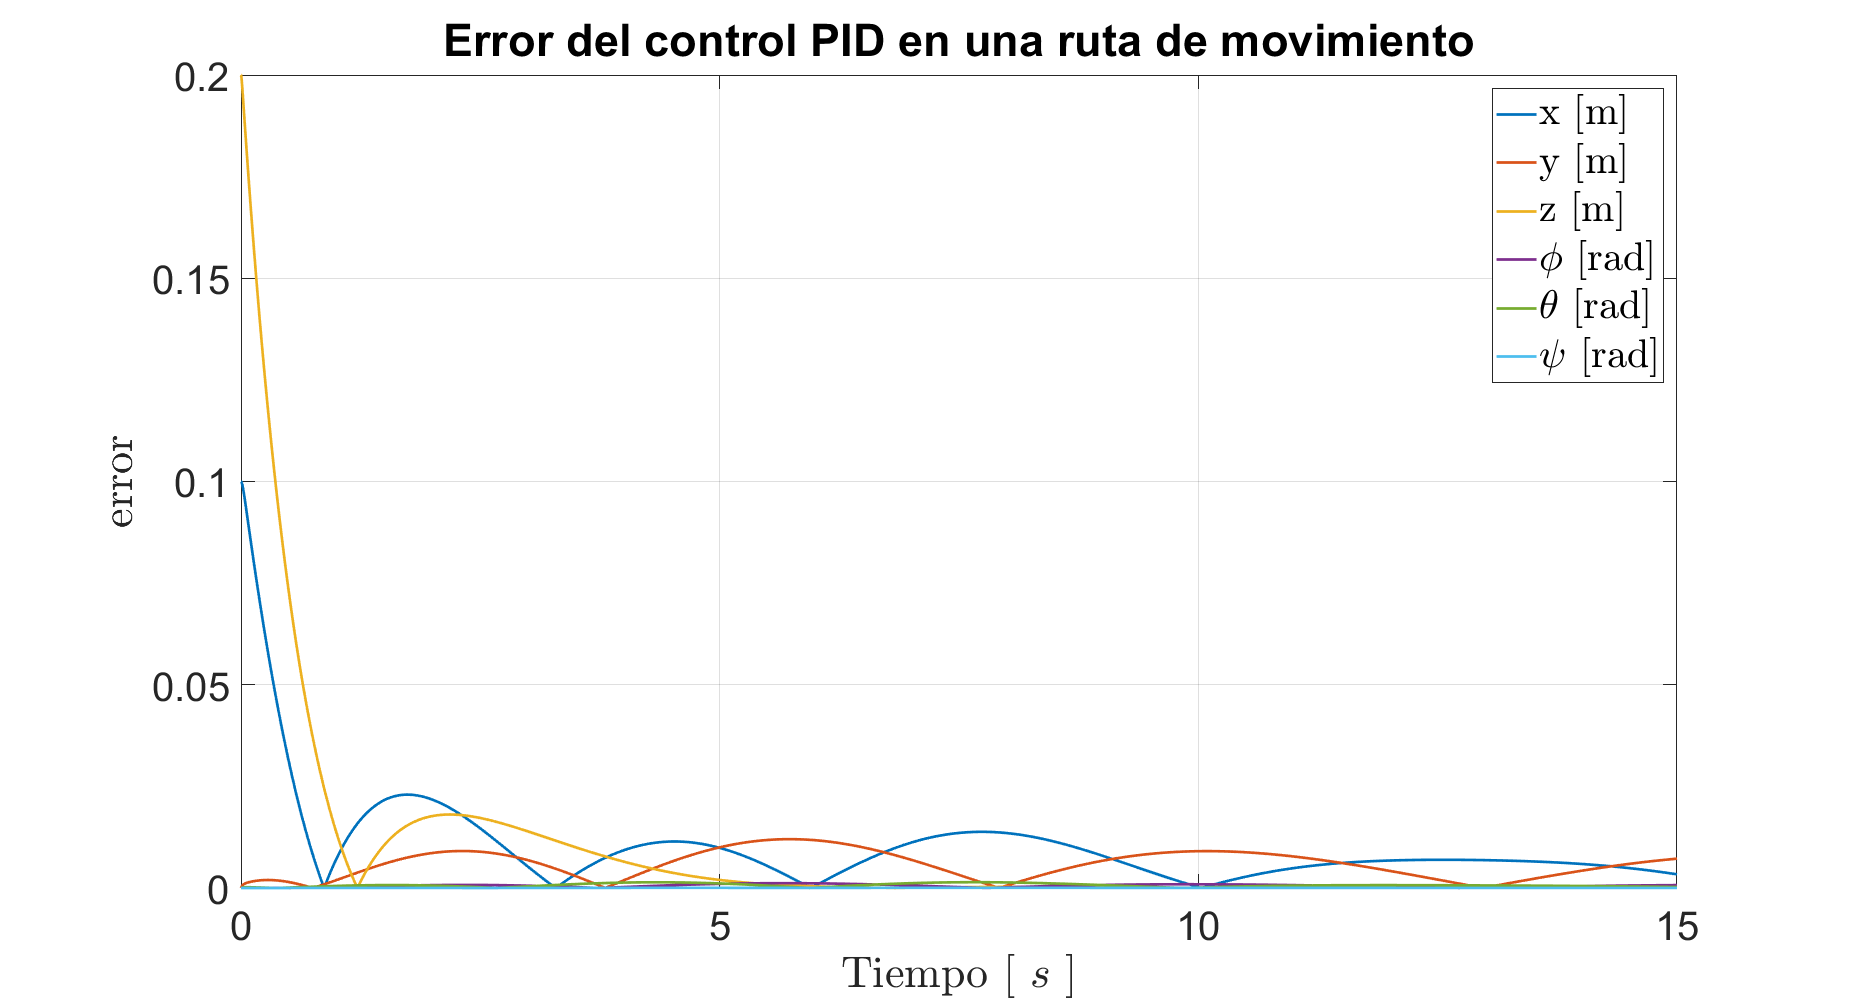
\includegraphics[width=0.4\textwidth]{errorPID.png}
    \caption{Error del sistema - PID.}
    \label{fig:PID error}
\end{figure}

\subsubsection{Bajo una referencia estática}

\subsubsection{Bajo patrón de movimiento}

\begin{figure}[htb]
    \centering
    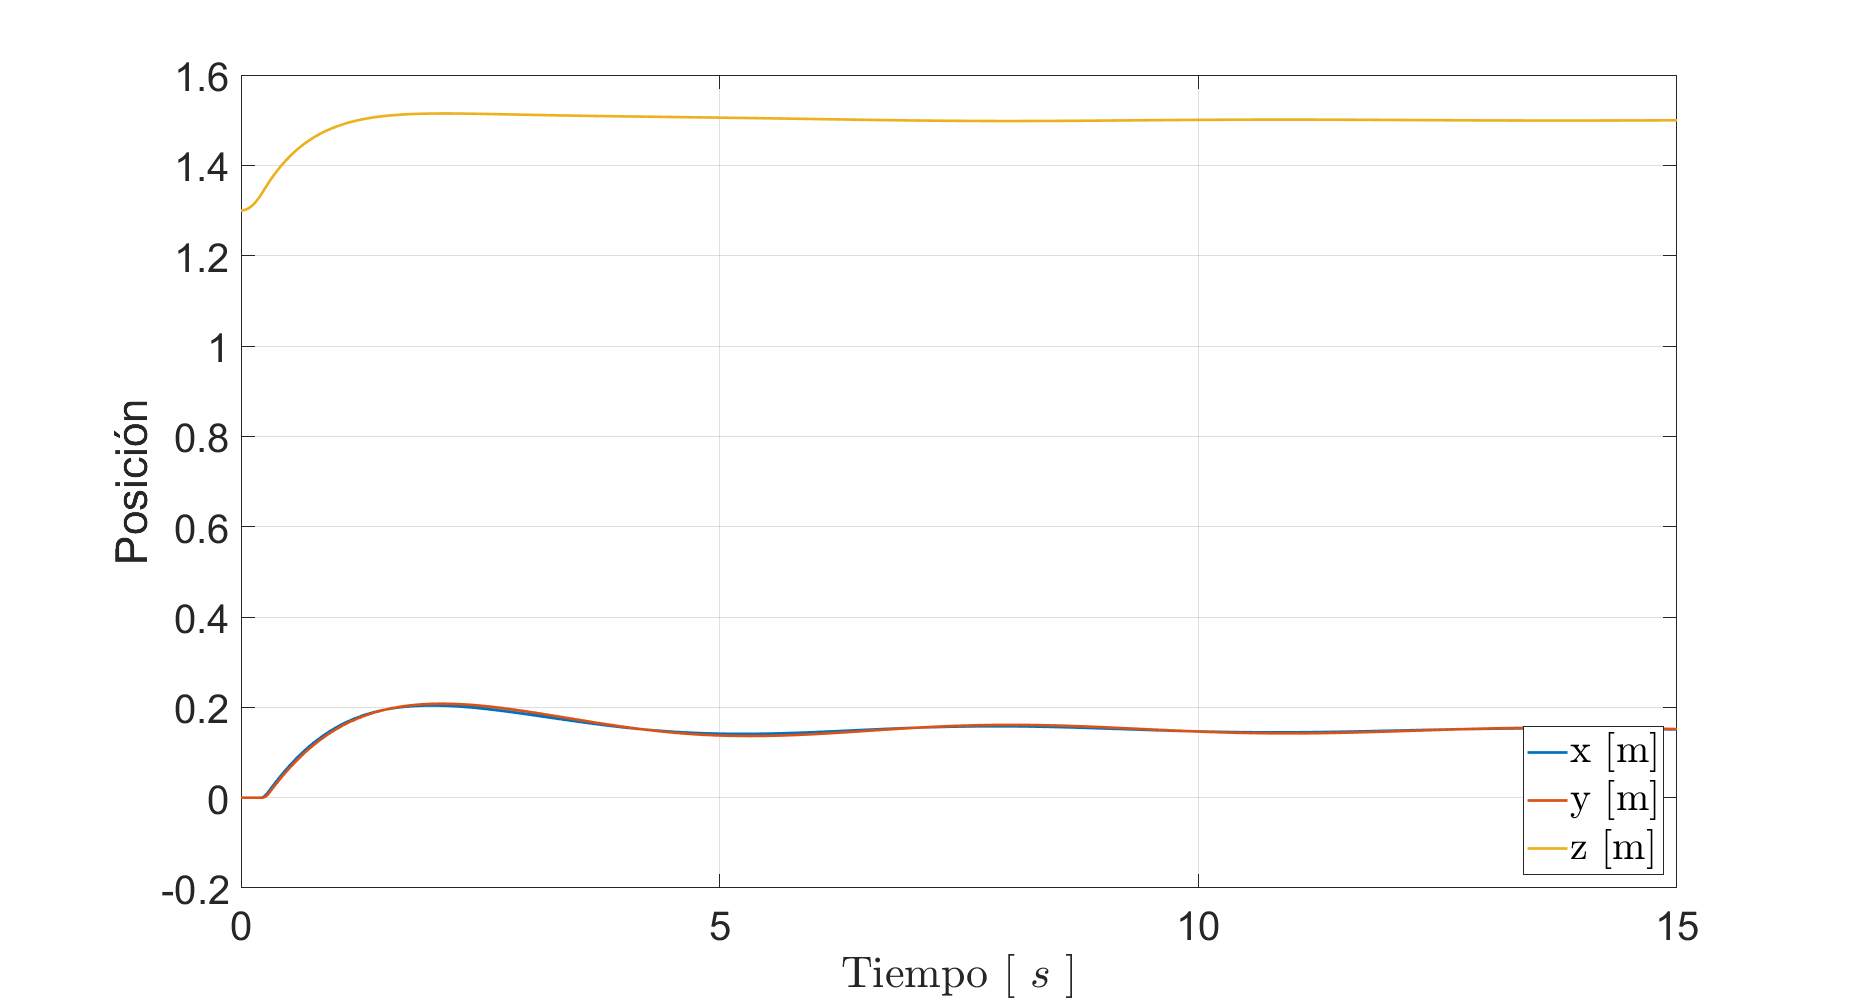
\includegraphics[width=0.4\textwidth]{posPIDe.png}
    \caption{Posición del sistema - PID.}
    \label{fig:PID position}
\end{figure}

\begin{figure}[htb]
    \centering
    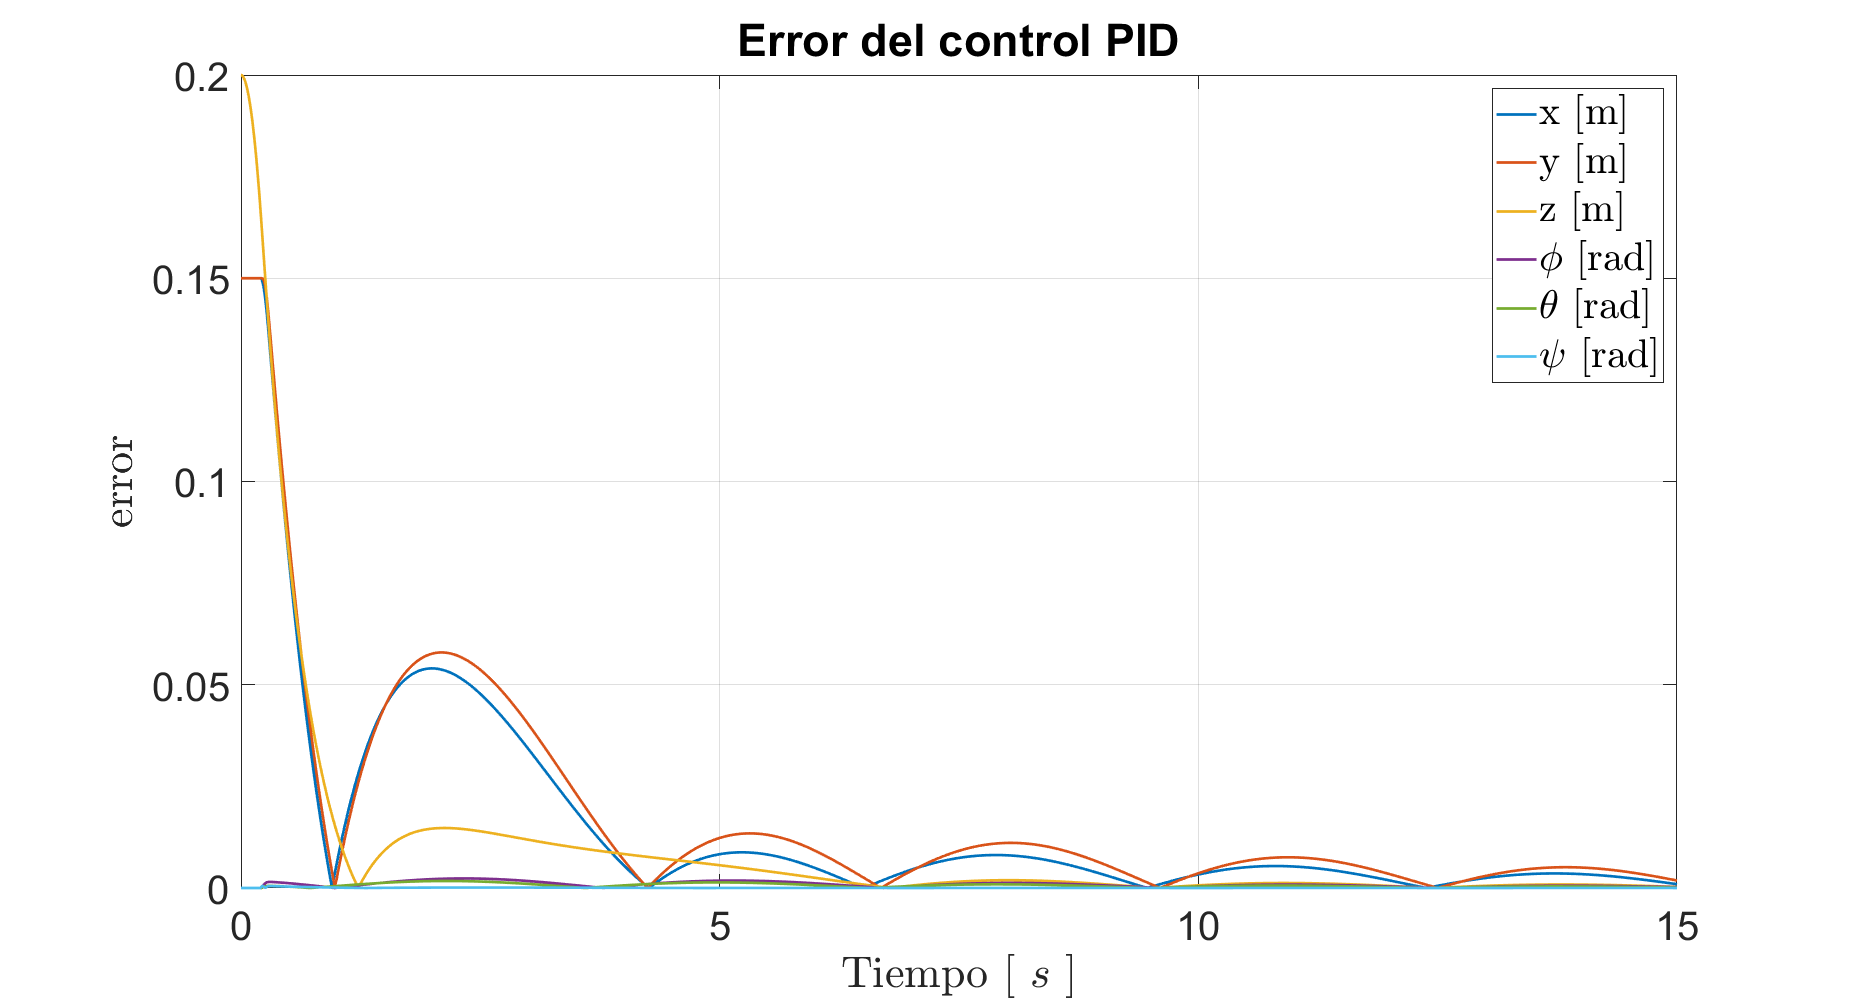
\includegraphics[width=0.4\textwidth]{errorPIDe.png}
    \caption{Error del sistema - PID.}
    \label{fig:PID error}
\end{figure}